\section{Adeline}

\subsection{Aufbau}

Im 1959 entwickelten der Stanford Professor Bernard Widrow und der Elektroingeneur Marcian Edward Hoff das sogenannte \emph{Adilne-Modell}. Der Name ist ein Akronym für \emph{ADAptive LINear Element}. Dieses Modell basiert auf dem Perceptron mit dem Unterschied, dass dieses Modell auf die Einheits-Sprungfunktion, wie sie das Peceptron verwendet, bei der Angleichung der Gewichte verzichtet. Es wird stattdessen eine lineare Aktivierungsfunktion $g(\mathbf{z})$ verwendet welche in diesem Fall erstmal mit der Identitätsfunktion besetzt wird (es gilt also $g(\mathbf{w}^T\mathbf{x}) = \mathbf{w}^T\mathbf{x}$). Außerdem wird eine Entscheidungsfunktion an das Ende des ganzen Modells gehängt um weiterhin die Werte quantifizieren zu können. Diese hat jedoch keinen Einfluss auf den Trainingsalgorithmus. 

\begin{figure}[!htb]
	\centering
	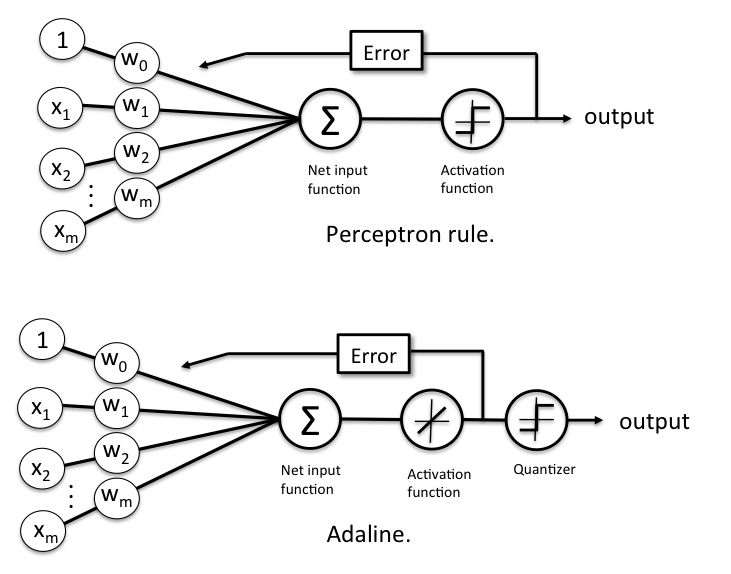
\includegraphics[width=.8\linewidth]{img/adeline_aufbau}
	\mycaption{Adeline - Aufbau}{mpNeuron}
	\label{fig:ad_aufbau}
\end{figure}


\subsection{Lernregel}

Widrow und Hoff definierten die Delta-Regel für den Lernalgorithmus ihres Modells. Dieser ist auch unter dem Namen \emph{Least-Mean-Square-Algorithmus} bekannt und ist auch heute noch von Relevanz). Im Kern möchte man hierbei das Minimum einer Kostenfunktion über dem Modell bestimmen. Ich werde im folgenden Abschnitt darauf eingehen wie dieser funktioniert und wie genau er für dieses Modell eingesetzt werden kann. 

todo Intro nochmal überarbeiten...

\paragraph{Gradientenverfahren}
Der wesentliche Nachteil der Einheits-Sprungfunktion ist der, dass sie nicht stetig und damit auch nicht differenzierbar ist. Deswegen hat man sich beim Lernalgorithmus des Adeline-Modells dazu entschieden stattdessen die Identitätsfunktion zu verwenden. 

Es wird zuerst eine Kostenfunktion $J(\mathbf{w})$ definiert die minimiert werden soll. Die Kostenfunktion wird durch die \emph{Regressionsquadratsumme} \footnote{engl. \emph{sum of squared errors} (SSE)} definiert. Die Formel sieh folgendermaßen aus: 

\begin{equation}
J(\mathbf{w})  = \frac{1}{2} \sum_{i} (\text{target}^{(i)} - \text{output}^{(i)})^2 \quad \quad \text{output}^{(i)} \in \mathbb{R} \\
\end{equation}

Wichtig hierbei, der Vorfaktor $ \frac{1}{2} $ gehört nicht zur herkömmlichen Regressionsquadratsumme, wurde hier jedoch hinzugefügt um später einfach ableiten zu können. Ziel ist es die bestimmte Abweichung über alle Trainingsdaten so minimal wie möglich zu gestalten. Dazu muss man die Gewichte sowie die Schwellwerte entsprechend anpassen. Um das zu tun reicht es das Minimum dieser Funktion zu finden. Dazu bedient man sich einer Technik namens \emph{Gradientenverfahren} (englisch \emph{gradient descent}). 

Werfen wir einen Blick auf die Abbildung \ref{fig:ad_gd1}. 

\begin{figure}[!htb]
	\centering
	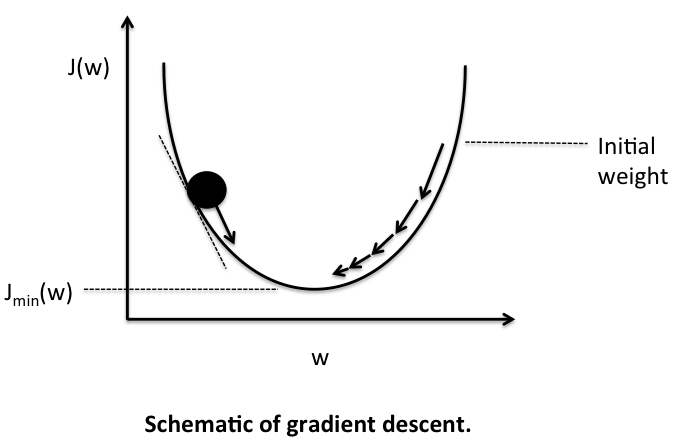
\includegraphics[width=.7\linewidth]{img/adeline_gd1}
	\mycaption{Gradientenverfahren mit eindimensionaler Kostenfunktion}{mpNeuron}
	\label{fig:ad_gd1}
\end{figure}

Die dargestellte Funktion besitzt nur einen Eingabewert. Zur Veranschaulichung kann man sich einen Ball vorstellen der einen Berg bzw. in ein Tal herunter rollt. Bezogen auf das Beispiel betrachtet man einen einen beliebigen Funktionswert und bestimmt die Ableitung an dieser Stelle. Diese Ableitung kann auch als \glqq Steigung \grqq an der betrachteten Stelle verstanden werden. Wenn man diese nun invertiert hat bekommt man theoretisch die \glqq Richtung \grqq in die der Ball rollen müsste. Ähnlich wie schon der Lernalgorithmus beim Perceptron wird mit einer Lernrate $\eta$ gearbeitet die bestimmt wie viel Veränderung in einem Iterations-Schritt stattfinden soll. Im Beispiel könnte man diese als Schrittweite verstehen. 
Wie weit in einem Schritt gearbeitet wird ist von fundamentaler Bedeutung. In Abbildung \ref{fig:ad_gd2} ist zu sehen, dass es problematisch sein kann die Lernrate zu hoch zu definieren denn der Algorithmus kann das Minimum auch überspringen. Andererseits kann es auch zu Problemen kommen wenn die Lernrate zu klein definiert wurde da der Algorithmus eventuell in einem lokalen Minimum \glqq steckenbleibt \grqq . Um gerade das erste Problem zu beheben wird die Lernrate heutzutage in jedem Iterationsschritt in Abhängigkeit der Größe der Steigung berechnet. 

\begin{figure}[!htb]
	\centering
	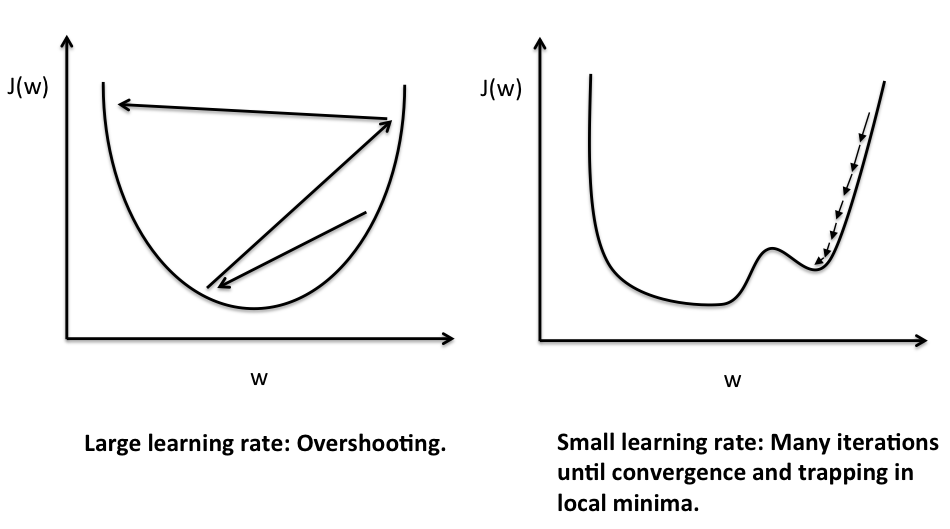
\includegraphics[width=\linewidth]{img/adeline_learning_rate}
	\mycaption{Gradientenverfahren - unterschiedliche Lernraten}{mpNeuron}
	\label{fig:ad_gd2}
\end{figure}

Letztendlich besitzt das hier betrachtete Modell aber meist mehr als ein einzelnes Gewicht weswegen man sich nun damit auseinander setzten muss wie man dieses Verfahren wohl auf eine Kostenfunktion mit einem mehrdimensionalen Vektor anpassen muss. Mit einem zweidimensionalen Eingabevektor ist dies noch relativ gut darstellbar (siehe Abbildung \ref{fig:ad_gd3}).

\begin{figure}[!htb]
	\centering
	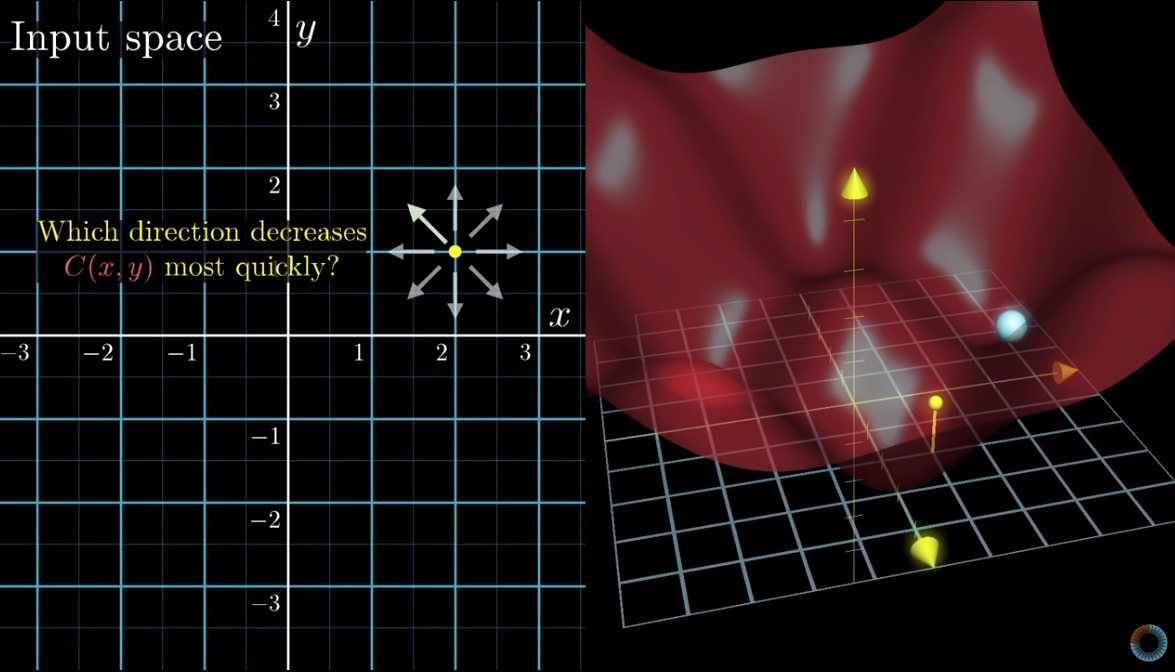
\includegraphics[width=\linewidth]{img/3dPlot_1}
	\mycaption{Gradientenverfahren - zweidimensionaler Eingabevektor}{mpNeuron}
	\label{fig:ad_gd3}
\end{figure}

Auch bei Funktionen mit mehreren Eingabewerten ist es möglich an einem betrachteten Eingabevektor die Steigung zu bestimmen, diese nennt sich hier jedoch \emph{Gradientenvektor}. Bei der gerade betrachteten Abbildung ist bilden die \emph{x} und die \emph{y-Achse} jeweils die beiden Eingabewerte der Funktion wobei die Ausgabe mit der \emph{z-Achse} dargestellt wird. Hier wird die Analogie mit dem Herabrollen eines Berges vielleicht noch etwas klarer. Auch hier gilt wie bei den anderen betrachteten Modellen wieder die Notation $w = w + \Delta w$. 

$\Delta w$ stellt den angedeutete Gradientenvektor dar. Im mehrdimensionalen Raum ist diese Gewichtsveränderung allgemein Fall für den kompletten Gewichtsvektor mit $\Delta \mathbf{w} = - \eta \nabla J(\mathbf{w})$ und für den speziellen Fall mit einem einzelnen Gewicht mit $\Delta w_j = - \eta \frac{\partial J}{\partial w_j}$ definiert. 

\subparagraph{Exkurs - Partielle Ableitungen} \cite{partAbl}
Da es sich im Beispiel um einen mehrdimensionalen Eingabevektor handelt muss man zum hierbei mit den partiellen Ableitungen arbeiten. Diese lassen sich am besten anhand eines weiteren Beispiels erklären. Betrachten wir zuerst einmal die Funktion $f(x, y) = x^2 + y^2$ (siehe Abbildung \ref{fig:partAbl1}). 

\begin{figure}[!htb]
	\centering
	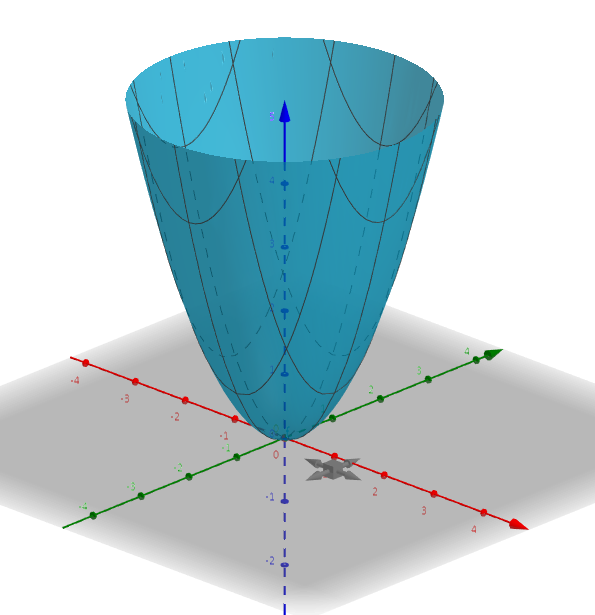
\includegraphics[width=.6\linewidth]{img/partAbl_1}
	\mycaption{Partielle Ableitung 1}{mpNeuron}
	\label{fig:partAbl1}
\end{figure}

todo



\FloatBarrier
Gegeben sei folgende Funktion \emph{f}: 


\subparagraph{Gradientenvektor bestimmen}